\begin{section}{Syntax and Semantics of Core SWIN}
\label{tw-fj}

Before explaining full SWIN for Java, which will
be discussed in Section~\ref{sec:extension}, we start with 
core SWIN for Featherweight Java~\cite{fj},
a known minimal core of Java. % Strictly speaking, 
% the transformation language for Featherweight Java is \emph{core} SWIN, and
% SWIN is for full Java. 
% If there is no confusion, in the follow text, we use
% SWIN for short.
If no confusion will be caused, we shall directly use SWIN to refer core SWIN.
We shall briefly review Featherweight Java, and 
explain the syntax and semantics of our transformation language SWIN for it.

\subsection{Background: Featherweight Java}
Featherweight Java (FJ for short) is a minimal core calculus for Java~\cite{fj}. 
FJ is small enough that a concise proof of type preserving
property is possible while it can be easily extended to full Java.

\begin{figure}[ht]
\begin{align*}
  & \mbox{Class Declaration}\\
  & \qquad\tt CL\ ::=\  \tt class\ C\ extends\ C \{\bar{C}\ \bar{f}; K\ \bar{M}\}\\
  & \mbox{Constructor Declaration}\\
  & \qquad\tt K \ ::=\  \tt C\ (\bar{C}\ \bar{f})\ \{ super(\bar{f}); this.\bar{f}=\bar{f}\}\\
  & \mbox{Method Declaration}\\
  & \qquad\tt M \ ::=\  \tt C\ m(\bar{C}\ \bar{x})\ \{ return\ t;\}\\
  & \mbox{Term}\\
  & \qquad\tt t \ ::=\  \tt x\ |\ t.f\ |\ t.m(\bar{t})\ |\ new\ C(\bar{t})\ |\ (C)\ t
\end{align*}
\caption{Syntax of Featherweight Java}
\label{fj-syntax}
\end{figure}
Figure~\ref{fj-syntax} shows the syntax of FJ.
The class declaration 
\[
\tt class\ C\ extends\ D\ \{\bar{C}\ \bar{f};\ K\ \bar{M}\}
\]
introduces a class named \verb|C| with superclass \verb|D|. The class has fields $\tt\bar{f}$ with types $\tt\bar{C}$,
a single constructor \verb|K|, and a suite of methods $\tt\bar{M}$.
%In the syntax of FJ, it abbreviate operations on pairs of
%sequences in the obvious way, 
In the formal notations, we use the bar notation adopted by Pierce~\cite{tpl} for repetitive elements: 
$\bar{a}$ to indicate a vector $a$,
and all operations defined on single values expand componentwisely to
vectors. For example, let $x_i$ be the $i$th element in $\bar{x}$, we
have $\bar{a}<\bar{b}$ is equal to $\forall i.\ a_i < b_i$ and $\bar{a}
\in S$ is equal to $\forall i.\ a_i \in S$.
Here, we write $\tt \bar{C}\ \bar{f}$ for $\tt C_{1}\,f_{1},\cdots,
C_{n}\,f_{n}$, where $\tt n$ is the length of $\tt\bar{C}$ and $\tt\bar{f}$.
Similarly, $\tt \bar{M};$ denotes $\tt M_1;\cdots ;M_n$, and $\tt \bar{M}$ 
denotes $\tt M_1\cdots M_n$.

The constructor declaration 
\[
\tt C(\bar{C}\,\bar{f})\{super(\bar{f});\,this.\bar{f}=\bar{f};\}
\]
defines the way to initialize a Java object, including a call to superclass constructor and assignments to class fields.

The method declaration 
\[
\tt C\ m(\bar{C}\ \bar{x})\{\ return\ t;\ \}
\]
introduces a method named $\tt m$ with return type $\tt C$ and
parameters $\tt \bar{x}$ of types $\tt\bar{C}$. The body of the method
is just a single term $\tt return\ t$.
%, and $\bar{x}$ is definition of
%bounded variables in $\tt t$.

There are only five terms in FJ, variable $\tt x$, field access $\tt
t.f$, method invocation $\tt t.m(\bar{t})$, object creation $\tt new\ 
C(\bar{e})$, and cast operation $\tt (C)e$. 
%There are no assignments,
%interfaces, overloading, messages to super, null pointers, base types,
%abstract method declarations, inner classes, etc.  
The  key
simplification in FJ is the omission of assignment. This implies that
an object's field is initialized by its constructor and never
changed afterwards. This restricts FJ to a ``functional'' fragment of
Java.
%, but is computationally complete as it is easy to encode
%lambda-calculus into it.

The typing rules of FJ are the same as those of plain
Java. One exception is that FJ does not support method
overloading. We refer the reader to the original paper~\cite{fj} and
Appendix~\ref{sec:FJTyping} for the typing rules. 

% \paragraph{APIs in Featherweight Java}
% \clmodify{}{Add this new section to introduce API in FJ}\todo{Revise this}

% As Featherweight Java is not a modular programming language,
% we define API in FJ as a bunch of class declarations in a FJ program and these class declarations are well type without refer to other class declarations.
% So an FJ program $\tt p=\bar{CL}$ can be divided into two parts: $\tt\overline{CL}_{API}$ and $\tt\overline{CL}_{client}$ (i.e. $\tt p = \overline{CL}_{API}~\overline{CL}_{client}$). 
% A transformation on a FJ program is to transform $\tt\overline{CL}_{client}$ and then replace $\tt\overline{CL}_{API}$ with new API class declarations $\tt\overline{CL}'_{API}$.
% The formal definition of the APIs in typing rules will be present later together with SWIN type checking systems.


\subsection{Core SWIN% : A Type-Safe Transformation Language
}

% SWIN is based on Twinning but with formal and more flexible
% semantics, which will be discussed here.
% In particular, SWIN employs a strict top-down order of rule
% applications, ensuring the transformation to be confluent and
% terminating. Furthermore, as will be seen in Section \ref{tw-type} later,
% SWIN also includes a set of typing
% rules checking the four conditions presented above. In the following
% sections we shall introduce SWIN formally and present our proof of
% type safety.
In this subsection we describe the syntax and evaluation rules of
SWIN formally. The type checking rules and the proof of type-safety property will be
presented in Section~\ref{tw-type} later.

\subsubsection{Syntax}

% SWIN is an update language specifying 
% how to transform client programs using old APIs to those using new APIs. 
The formal definition of SWIN is presented
in Figure~\ref{syntaxofuc}. Simiarly to Twinning, a SWIN program $\tt\Pi$ is a set of 
transformation rules, and a transformation rule ($\tt\pi=(\bar{d})\ [l:C_l\ \rightarrow\ r:C_r]$) consists of three
parts: 1) meta variable declarations ($\tt \bar{d}$), 2) left hand side source
code pattern ($\tt l$) and 3) right hand side target code pattern ($\tt r$). 
Source code pattern $\tt l$ will be used to match an expression in old client program,
and target code pattern $\tt r$ is an FJ term use a new API with meta-variables bounded in $\tt d$
which is used to generate updated client code. And the variable declaration part
($\tt d=x:A\hookrightarrow B$) associates a metavariable with its type migration information: $\tt x$ is of type $\tt A$ in $\tt l$ and of type $\tt B$ in $\tt r$.

\begin{figure}
\begin{align*}
  \tt \Pi \quad ::=\quad  &\tt  \{\bar\pi\}                     &\text{Transformation program}\\
  \tt \pi \quad ::=\quad  &\tt  (\bar{d})\ [l\ \rightarrow\ r]    &\text{Rule}\\
  \tt d   \quad ::=\quad  &\tt  x:C_1\hookrightarrow C_2          & \text{Variable declaration}\\
  \tt l   \quad ::=\quad  &\tt  x.f ~ | ~ new\ C(\bar{x}) ~|~ x.m(\bar{x})  & \text{Code pattern}\\
  \tt r   \quad ::=\quad  &\tt  t                                 &\text{FJ term}
\end{align*}
%Variables in $\tt r$ are meta-variables bounded by the variable definition in $\pi$.
\caption{Syntax of SWIN}
\label{syntaxofuc}
\end{figure}

An informal explanation of the rule can be seen from its correspondence 
with the replacement rule in Section \ref{sec:examples}. 
For example, the mapping rule
\[
\tt
\pi=(x:A\hookrightarrow
L,y:B\hookrightarrow M)\ [\ x.m(y):C \rightarrow x.h(y):D\ ]
\]
can be seen as the following replacement rule:
\begin{quote}
\begin{lstlisting}
[ 
 C (A x, B y) { return x.m(y); }
 D (L x, M y) { return x.h(y); }
]
\end{lstlisting}
\end{quote}
%The first part $\tt x.m(y)$ means that the source pattern is a Java
%term of invocation.  The method name is $\tt m$ and it is a method of
%object $\tt x$, which is an object of class $\tt A$ according to the
%variable declaration $\tt x:A\hookrightarrow L$ part of the rule.  The
%declaration $\tt y:B\hookrightarrow M$ and the appearence of $\tt y$
%in $\tt x.m(y)$ indicates the method $\tt m$ has only one argument of
%type $\tt B$.  
Now if there is a client source code term $\tt
(new\ A()).m(new\ B())$, the rule will match the term as \verb|x| binds to
$\tt new\ A()$, \verb|y| binds to $\tt new\ B()$, and the method name
$\tt m$ matches the method name in the term. It results in that the updated term
$\tt (new\ A()).h(new\ B())$ is of type $D$.
Note that this rule 
does not match the term $\tt (new\ C()).m(new\ B())$, as the type
of the variable $\tt x$ (type $\tt A$) does not
match the type of the term $\tt new\ C()$ (type $\tt C$).  
%The third
%part $\tt x.h(y)$ of $\pi$ is the target code pattern, which will be
%used to generate new client code with meta-variable substitution and
%it will be introduced in the next part.  
%
% One thing we need to take care about is the variable declaration part
% of a rule $\tt \pi$.  
% Note also that in a mapping rule, there may be variables
% appearing in both source code pattern and target code pattern, and all
% these variables should be specified in the variable declaration part.
% A declaration for $x:A\hookrightarrow B$ means that in source code
% pattern $\tt l$, $\tt x$ has type $\tt A$ and in target code pattern
% $\tt r$, $\tt x$ has type $\tt B$, and these $\tt x$ are exactly the
% same. It is defined in this way as when we apply the rule to a
% piece of client code, a matching of source code pattern will generate
% a substitution of $\tt x\rightarrow t$, which will be used to instantiate
% $\tt x$ in target code pattern with $\tt t$ and generate new client
% code.

To ensure convergence, we do not allow the left hand sides of
two rules to match the same method or the same constructor. In this
way we can ensure one term is matched by at most one rule, resulting
in a unique result after transformation.
% Furthermore, for the ease of presentation, we do not allow a rule 
% to replace a field access in the SWIN for FJ, 
% such as replacing \code{t.f} with \code{t.m()}.
% This feature can be easily implemented by treating a field as a method
% without parameter in FJ, because FJ does not allow
% the writing of an API field in the user code while the initialization
% of a field is inside an API itself and does not need to be
% transformed. Yet in full Java, supporting fields needs some more work,
% as will be discussed in Section~\ref{sec:extension}.


\subsubsection{Semantics: Evaluation Rules}

We assume that an FJ program, which is a set of class declarations, can be divided into two parts: 
$\tt\{\overline{CL}_{API}\}$ and $\tt\{\overline{CL}_{client}\}$,
where $\tt\overline{CL}_{API}$ is the source API,
consisting of class definitions that are
type-correct by themselves; $\tt\overline{CL}_{client}$ is the client
program to be transformed, consisting of class definitions that depends on $\tt\overline{CL}_{API}$. A
transformation on an FJ program is to apply the transformation rules on 
$\tt\overline{CL}_{client}$ to get $\tt\overline{CL}'_{client}$, and then replace $\tt\overline{CL}_{API}$
with the target API $\tt\overline{CL}'_{API}$, such that
$\tt\overline{CL}'_{API}$ and $\tt\overline{CL}'_{client}$ form a
type-correct program. 

In formal notations, we define $\tt API$ to denote $\{~\overline{CL}~\}$, and operations on $\tt API$s are naturally set operations (e.g. $\tt API_1-API_2$ is set substraction, which will exclude class declarations in $\tt API_2$ from $\tt API_1$). In particular, we use the notation $\tt API_s$ to denote the
source API, $\tt\overline{CL}_{API}$, and $\tt API_d$ to denote the target
API, $\tt\overline{CL}'_{API}$, respectively. 

% As Featherweight Java is not a modular programming language,
% we define API in FJ as a bunch of class declarations in a FJ program and these class declarations are well type without refer to other class declarations.
% So an FJ program $\tt p=\bar{CL}$ can be divided into two parts: $\tt\overline{CL}_{API}$ and $\tt\overline{CL}_{client}$ (i.e. $\tt p = \overline{CL}_{API}~\overline{CL}_{client}$). 
% A transformation on a FJ program is to transform $\tt\overline{CL}_{client}$ and then replace $\tt\overline{CL}_{API}$ with new API class declarations $\tt\overline{CL}'_{API}$.
% The formal definition of the APIs in typing rules will be present later together with SWIN type checking systems.



\begin{figure*}[htb!]
\begin{center}
\AXC{$\tt CL=class\ C_{1}\ extends\ C_2\ \{\ \bar{C}\ \bar{f};\ K\ \bar{M}\ \}$}                             \RightLabel{~(E-DECLARATION)}
\UIC{$\tt \Pi(CL)= class\ \Pi(C_1)\ extends\ \Pi(C_2)\ \{\ \Pi(\bar{C})\ \bar{f};\ \Pi(K)\  \overline{\Pi(M)}\ \}$}
\DP
\end{center}
\vspace{2pt}

\begin{center}
\AXC{$\tt K=C_1\ (\bar{C}_2\ \bar{f}_2)\ \{super(\bar{f}_3);\ this.\bar{f}_i=\bar{f}_j\}$}                             \RightLabel{~(E-CONSTRUCTOR)}
\UIC{$\tt \Pi(K)=\Pi(C_1)\ (\Pi(\bar{C}_2)\ \bar{f}_2)\ \{super(\bar{f}_3);\ this.\bar{f}_i=\bar{f}_j\}$}
\DP
\end{center}
\vspace{2pt}

\begin{center}
\AXC{$\tt M=C_1\ m(\bar{C}\ \bar{x})\ \{return\ t;\}$}                             
\RightLabel{~(E-METHOD)}
\UIC{$\tt\Pi(M)=\Pi(C_1)\ m(\Pi(\bar{C})\ \bar{x})\ \{return\ \Pi(t);\}$}
\AXC{$\tt C_0\hookrightarrow C_1\in \mathbf{TypeMapping}(\Pi)$}                             
\RightLabel{~(E-CLASS)}
\UIC{$\tt \Pi(C_0)=C_1$}
\noLine
\BIC{}
\DP
\end{center}
\vspace{2pt}

\begin{center}
\AXC{$\tt \forall C.~C_0\hookrightarrow C\notin \mathbf{TypeMapping}(\Pi)$}
\RightLabel{~(E-ALTER-CLASS)}
\UIC{$\tt \Pi(C_0)=C_0$}
\AXC{}                 \RightLabel{~(E-T-VALUE)}
\UIC{$\tt \Pi(x)=x$}
\noLine
\BIC{}
\DP
\end{center}
\vspace{2pt}

\begin{center}
\AXC{$\tt (x:C_1\hookrightarrow C_2)[~x.f:C\ \rightarrow\ r:D~]\in \Pi$ ~~~~ $\tt\type{t} <: C_1$}                 \RightLabel{~(E-T-FIELD)}
\UIC{$\tt \Pi(t.f)=\tt[~x\rightarrow \Pi(t)~]r$}
\DP
\end{center}
\vspace{2pt}

\begin{center}
\AXC{}      \RightLabel{~(E-T-CAST)}
\UIC{$\tt \Pi((C)\ t)=(\Pi(C))\ \Pi(t)$}
%%% the next rule
\AXC{$\tt (\bar{d})[\ new\ C_0(\ \bar{x}\ ):C\ \rightarrow\ r:D]\in \Pi$}
\noLine
\UIC{$\tt\quad\quad \{~\bar{x}:\overline{C_1\hookrightarrow C_2}~\}\subseteq \bar{d} \quad\quad  \type{\bar{t}_u}<:\bar{C}_1$}               
\RightLabel{~(E-T-NEW)}
\UIC{$\tt \Pi(new\ C_0(\bar{t}_u))=[~\bar{x}\rightarrow \overline{\Pi(t_u)}~](r)$}
\noLine
\BIC{}
\DP
\end{center}
\vspace{2pt}

\begin{center}
\AXC{$\tt  (\bar{d})[\ x_0.m_0(\ \overline{y}\ ):C\ \rightarrow\ r:D]\in\Pi$}
\noLine
\UIC{$\tt \{\bar{y}:\overline{C_1\hookrightarrow C_2},\ x_0:C_3\hookrightarrow C_4\} \subseteq \bar{d} \quad\quad\type{t_0}<:C_3\quad\quad \type{\bar{t}_u}<:\bar{C}_1$}\RightLabel{~(E-T-INVOKE)}
\UIC{$\tt \Pi(t_0.m_0(\bar{t}_u))=[~x_0\rightarrow \Pi(t_0),\ \bar{y}\rightarrow \overline{\Pi(t_u)}~](r)$}
\DP
\end{center}
\vspace{2pt}

\begin{center}
\AXC{$\mbox{\tt no other inference rule can be applied}$}   
\RightLabel{~(E-ALTER-NEW)}
\UIC{$\tt \Pi(new\ C_0(\bar{t}_u))=new\ C_0(~\overline{\Pi(t_u)}~)$}
\DP
\end{center}
\vspace{2pt}

\begin{center}
\AXC{$\mbox{\tt no other inference rule can be applied}$}   
\RightLabel{~(E-ALTER-INVOKE)}
\UIC{$\tt \Pi(t_0.m_0(\bar{t}_u))=\Pi(t_0).m(~\overline{\Pi(t_u)}~)$}
\DP
\end{center}
\vspace{2pt}

\begin{center}
\AXC{$\mbox{\tt no other inference rule can be applied}$}                 \RightLabel{~(E-ALTER-FIELD)}
\UIC{$\tt \Pi(t.f)=\tt\Pi(t).f$}
\DP
\end{center}
\vspace{2pt}
\caption{Evaluation Rules of SWIN}
\label{semanticsofuc}
\end{figure*}

\begin{figure*}
\begin{align*}  
&\tt \mathbf{TypeMapping}([(~\bar{x}:\overline{C_1\hookrightarrow C_2}~)\ [l:C\ \rightarrow\ r:D]]) = \{C\hookrightarrow D\}\cup\{~\overline{C_1\hookrightarrow C_2}~\}\\
&\tt \mathbf{TypeMapping}(\{\bar{\pi}\}) = \bigcup_{\pi}~(\mathbf{TypeMapping}(\pi)) ~~~~~~ \text{(Extract type migration information)}\\
&\tt \mathbf{Decl}(class~C~extends~D~\{...\}) = C   ~~~~~~
\text{(Extract the declared class name)}
% ~~~~~~
% \AXC{$\tt \vdash_{FJ}^{API_S} t : C$}
% \RightLabel{~(Get the type of a term)}
% \UIC{$\tt {Type}(t)=C$}
% \DP
\end{align*}
\caption{Auxiliary Functions used in Figure~\ref{semanticsofuc} and Figure~\ref{logicrules}}
\label{auxiliarydefofuc}
\end{figure*}

%This part defines rules of how to update Java client code with SWIN code.\par
%informally explained the meaning of mapping rules.
Figure~\ref{semanticsofuc} summarizes the formal semantics of SWIN.
In the rules, $\tt A <: B$ indicates that \code{A} is a subtype of \code{B}. A transformation program $\tt\Pi$ is formalized as a transformation from 
source code to target code on both types and terms. This transformation consists of the following three steps.

\begin{enumerate}
\item {\em Transformation Promotion}: The first three rules \\(E-DECLARATION, E-CONSTRUCTOR, E-METHOD)
are used to promote $\tt\Pi$ up to types and terms through a class declaration, a
construction definition, and a method definition, respectively.

\item {\em Type Transformation}: The next E-CLASS rule is used to transform source types in the source API to target types in target API
  based on the type mappings defined in $\tt\Pi$. Those types which
  are not involved in type mapping of $\tt \Pi$ will stay the same
  according to the rule E-ALTER-CLASS. An important components of the
  two rules is \textbf{TypeMapping}, which records how types in $\tt
  API_s$ is mapped to $\tt API_d$ by the transformation program, and
  is defined in Figure~\ref{auxiliarydefofuc}.
  
  % The rules for extracting type migration information from $\tt\Pi$ can be referred to \textbf{TypeMapping} in Figure~\ref{auxiliarydefofuc}.

\item {\em Term Transformation}: The rest of the rules are used to
  transform source code terms. As the syntactic definitions in
  Figure~\ref{syntaxofuc} show, an FJ term takes five forms. The form
  $\tt x$ and $\tt (C)t$ are dealt by E-T-VALUE and E-T-CAST,
  respectively, which basically further applies $\Pi$ to sub terms.
  The other three forms are dealt by E-T-FIELD, E-T-NEW, E-T-INVOKE,
  respectively. The three evaluation rules apply matched SWIN transformation
  rules to the current term. In case no rule can be applied,
  evaluation rules E-ALTER-FIELD, E-ALTER-INVOKE, E-ALTER-NEW apply
  $\Pi$ sub terms. In the definitions, we use $\tt Type(t)$ to get the
  type of a term $\tt t$ based on FJ typing rules.
%   ; $\tt\Pi$ is recursively applied to subterms and 
% its rules are used to transform $\tt new\ C_0(\bar{t}_u)$ or $\tt t_0.m_0(\bar{t}_u)$ or $\tt t.f$ whenever possible.
% When reaching $\tt new\ C_0(\bar{t}_u)$, if there is a rule 
% with the source pattern of the form $\tt new\ C_0(\ \bar{x}\ )$ and the type of $\tt \bar{t}_u$ is a subtype
% of that of $\tt \bar{x}$, it will apply the rule on the term by replacing meta-variables $\tt \bar{x}$ in the target code pattern $\tt r$ by corresponding $\tt \Pi(\bar{t}_u)$ (based on E-T-NEW), otherwise 
% $\tt \Pi$ is recursively applied to its subterm (based on
% E-ALTER-NEW). The cases for $\tt t_0.m_0(\bar{t}_u)$ and $\tt t.f$
% is dealt with similarly.

  
\end{enumerate}

%
%An update body $\tt\Pi$ will transform both types and terms in source code. 
%When we apply $\tt\Pi$ on Java source code,
%generally we have three steps:
%\begin{enumerate}
%\item Match the term with a rule $\tt\pi$ in $\tt\Pi$.
%\item Generate a substitution of meta-variables to Java term based on the matching.
%\item Transform the target code pattern $\tt r$ to Java client code by meta-variables substituti%on.
%\end{enumerate}
%\par

To be concrete, let us see an example. Suppose that we want to switch from 
the old API ($\tt API_s$) to a new one ($\tt API_d$)\footnote{
We omit the API method bodies here as it is not necessary
to see the details of how an API method is implemented;
it is sufficient to show the input types and the return type of each method in API.}
\[
\begin{array}{lll}
\mbox{$\tt API_s=\{class\ A\ \{\ A()\{...\};\ A\ h(A\ a)\{...\};\};\}$}\\
\mbox{$\tt API_d=\{class\ B\ \{\ B()\{...\};\ B\ k(B\ b,B\ c)\{...\};\};\}$}
\end{array}
\]
and we use the following SWIN transformation program
\[
\begin{array}{lll}
\mbox{$\tt\Pi=[\pi_1,\pi_2]$}\\
{\bf where}\\
\quad \mbox{$\tt\pi_1=()\ [\ new\ A() : A \rightarrow new\ B() : B\ ]$}\\
\quad \mbox{$\tt\pi_2=(x:A\hookrightarrow B, u:A\hookrightarrow B)$} \\
\qquad\qquad \mbox{$\tt[\ x.h(u) : A \rightarrow x.k(u,new\ B()) : B\ ]$}
\end{array}
\]
to transform the following source client Java code.
\[
\mbox{$\tt(new\ A()).h(new\ A())$}
\]
The transformation is done as follows.
\[
\begin{array}{llll}
   & \mbox{$\tt \Pi((new\ A()).h(new\ A())$}\\
=  & \reason{by E-T-INVOKE with rule $\pi_2$}\\
   & \mbox{$\tt [x\rightarrow \Pi(new\ A()), u\rightarrow \Pi(new\ A())](x.k(u,new\ B()) )$}\\
=  & \reason{replace $\tt x$ and $\tt u$ in $\tt x.k(u,new\ B())$ }\\
   & \mbox{$\tt \Pi(new\ A()).k( \Pi(new\ A()),new\ B())$}\\
=  & \reason{by E-T-NEW with rule $\pi_1$}\\
   & \mbox{$\tt [~](new\ B()).k( [~](new\ B()),new\ B())$}\\
=  & \reason{ since $\tt [~](new\ B()) = new\ B()$ }\\
   & \mbox{$\tt new\ B().k(new\ B(),new\ B())$}\\
\end{array}
\]
Thus it results in target code $\tt new\ B().k(new\ B(),new\ B())$.

% \subsubsection{Evaluation Property: Convergence}

\smallskip
Our evaluation rules ensure the convergence of any SWIN program, which
is discussed in the following theorem and its proof sketch.
\begin{theorem}
  Any SWIN program is convergent.
\end{theorem}
\begin{proof-sketch}
%\clmodify{$\emptyset$}{new section to introduce action property}
%When a SWIN program acts on a FJ term, it recursively visit the sub terms
%of that term, and for each visit, the transformation will be applied
%on the original term, and produce the transformation result by
%combining the transformed sub terms. 
SWIN employs a normal order evaluation semantics. First, the evaluation rules visit
a term leftmost and outermost. After performing the transformation on that term, the evaluation 
rules recursively visit the sub terms of the term, and for each visit, the transformation
will be applied on the original sub terms, and produce the transformation result by combining
the transformed sub terms. 
In this way we can ensure each recursive visit will be 
terminated as the length of the sub terms 
are always shorter than the term. Also, we can ensure the transformation on a term
is confluence, as each program element is exactly transformed once. % In a word, SWIN is \mbox{\emph{convergent}}.
\end{proof-sketch}
\end{section}
%When we first apply $\Pi$ on the source code, we know the source code is a term of the form $\tt t.m(\bar{t})$. Thus we use the rule E-T-INVOKE to transform the term.
%\par
%We have $\pi_2$ to match the term and the matching is: $$\{\tt new\ A()\leftrightarrow x, h\leftrightarrow h, new\ A()\leftrightarrow u\}$$
%We now can generate an substitution of meta-variables according to the rule. Then we have the following substitution:$$\tt \{x\rightarrow \Pi(new\ A()), u\rightarrow \Pi(new\ A())\}$$
%With the update language applied recursively one the term, we have a final substitution $$\tt \{x\rightarrow new\ B(), u\rightarrow new\ B()\}$$. The last step is the application of the substitution on the target code pattern $\tt x.k(u,new\ B())$ in the rule $\pi_2$. We translate all meta-variables to Java terms and generate the updated source code.$$\tt(new\ B()).k(new\ B(),new\ B());$$
%The update process is displayed in Figure \ref{exofuc} \todo{need to update the figure}.
%\begin{figure}[ht]
%\centering
%    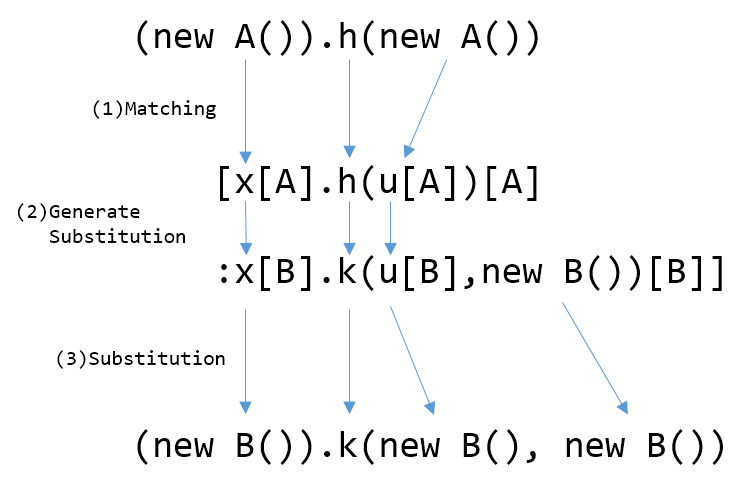
\includegraphics[width=6cm]{example1.png}
%    \caption{An example}
%    \label{exofuc}
%\end{figure}
%\par
%Other evaluation rules are similar to the rule E-INVOKE. And in some cases, a Java term may not be matched by any of the rules and we have E-ALTER-NEW and E-ALTER-INVOKE to transform the code. For E-CLASS, we can easily translate a class name in old API to a class name in new API if there is a type mapping specified in the SWIN body $\tt \Pi$.


%%% Local Variables: 
%%% mode: latex
%%% TeX-master: "pepm-15"
%%% End: 
